\section{Lab resultater og analyse}
I laben vi gjennomførte, undersøkte vi hvordan et firkant-pulstog påvirkes når det sendes gjennom en koaksialkabel av 2 lengder 5m og 30m. Ideellt sett skulle man hatt brukt Ethernet-kabeler, men pga manglende tilgang brukte vi koaksialkabeler. Noe som var tilstrekkelig for å illustrere fenomenene vi ønsket å studere.

\subsection{Utstyr/innstillinger}
Utstyret vi brukte i laben inkluderte:
\begin{itemize}
    \item Funksjonsgenerator: For å generere firkant-pulstoget med ønsket periode, amplitude og startfase.
    \begin{itemize}
        \item Periode: $T = 2 \mu s$ 
        \item Amplitude: $2.5V_{pp}$
        \item Startfase: $0\si{\degree}$ (slik at signalet starter ved null)
        \item Duty-cycle: 50\%
        \item Signalform: Firkant
    \end{itemize}
    \item Oscilloskop: For å måle inngangs-, utgangssignaler og FFT.
    \item Koaksialkabeler: Tre kabler med lengder på 5m og 30m (impedans 50 ohm).
\end{itemize}
\subsection{5m koaksialkabel}
\subsubsection{Tidsdomenet}
Figur \ref{fig:lab5m_time} viser inngangs- og utgangssignalene for 5m koaksialkabel i tidsdomenet. Utgangssignalet er tilnærmet identisk med inngangssignalet, med kun minimal demping og faseforskyvning. Dette indikerer en nesten ideell, ikke-dispersiv oppførsel, der signalet hovedsakelig påvirkes av en tidsforsinkelse uten merkbar forvrengning eller tap. Dette er forventet, ettersom kabelen er relativt kort og dermed introduserer svært små tap.
\begin{figure}[h]
    \centering
    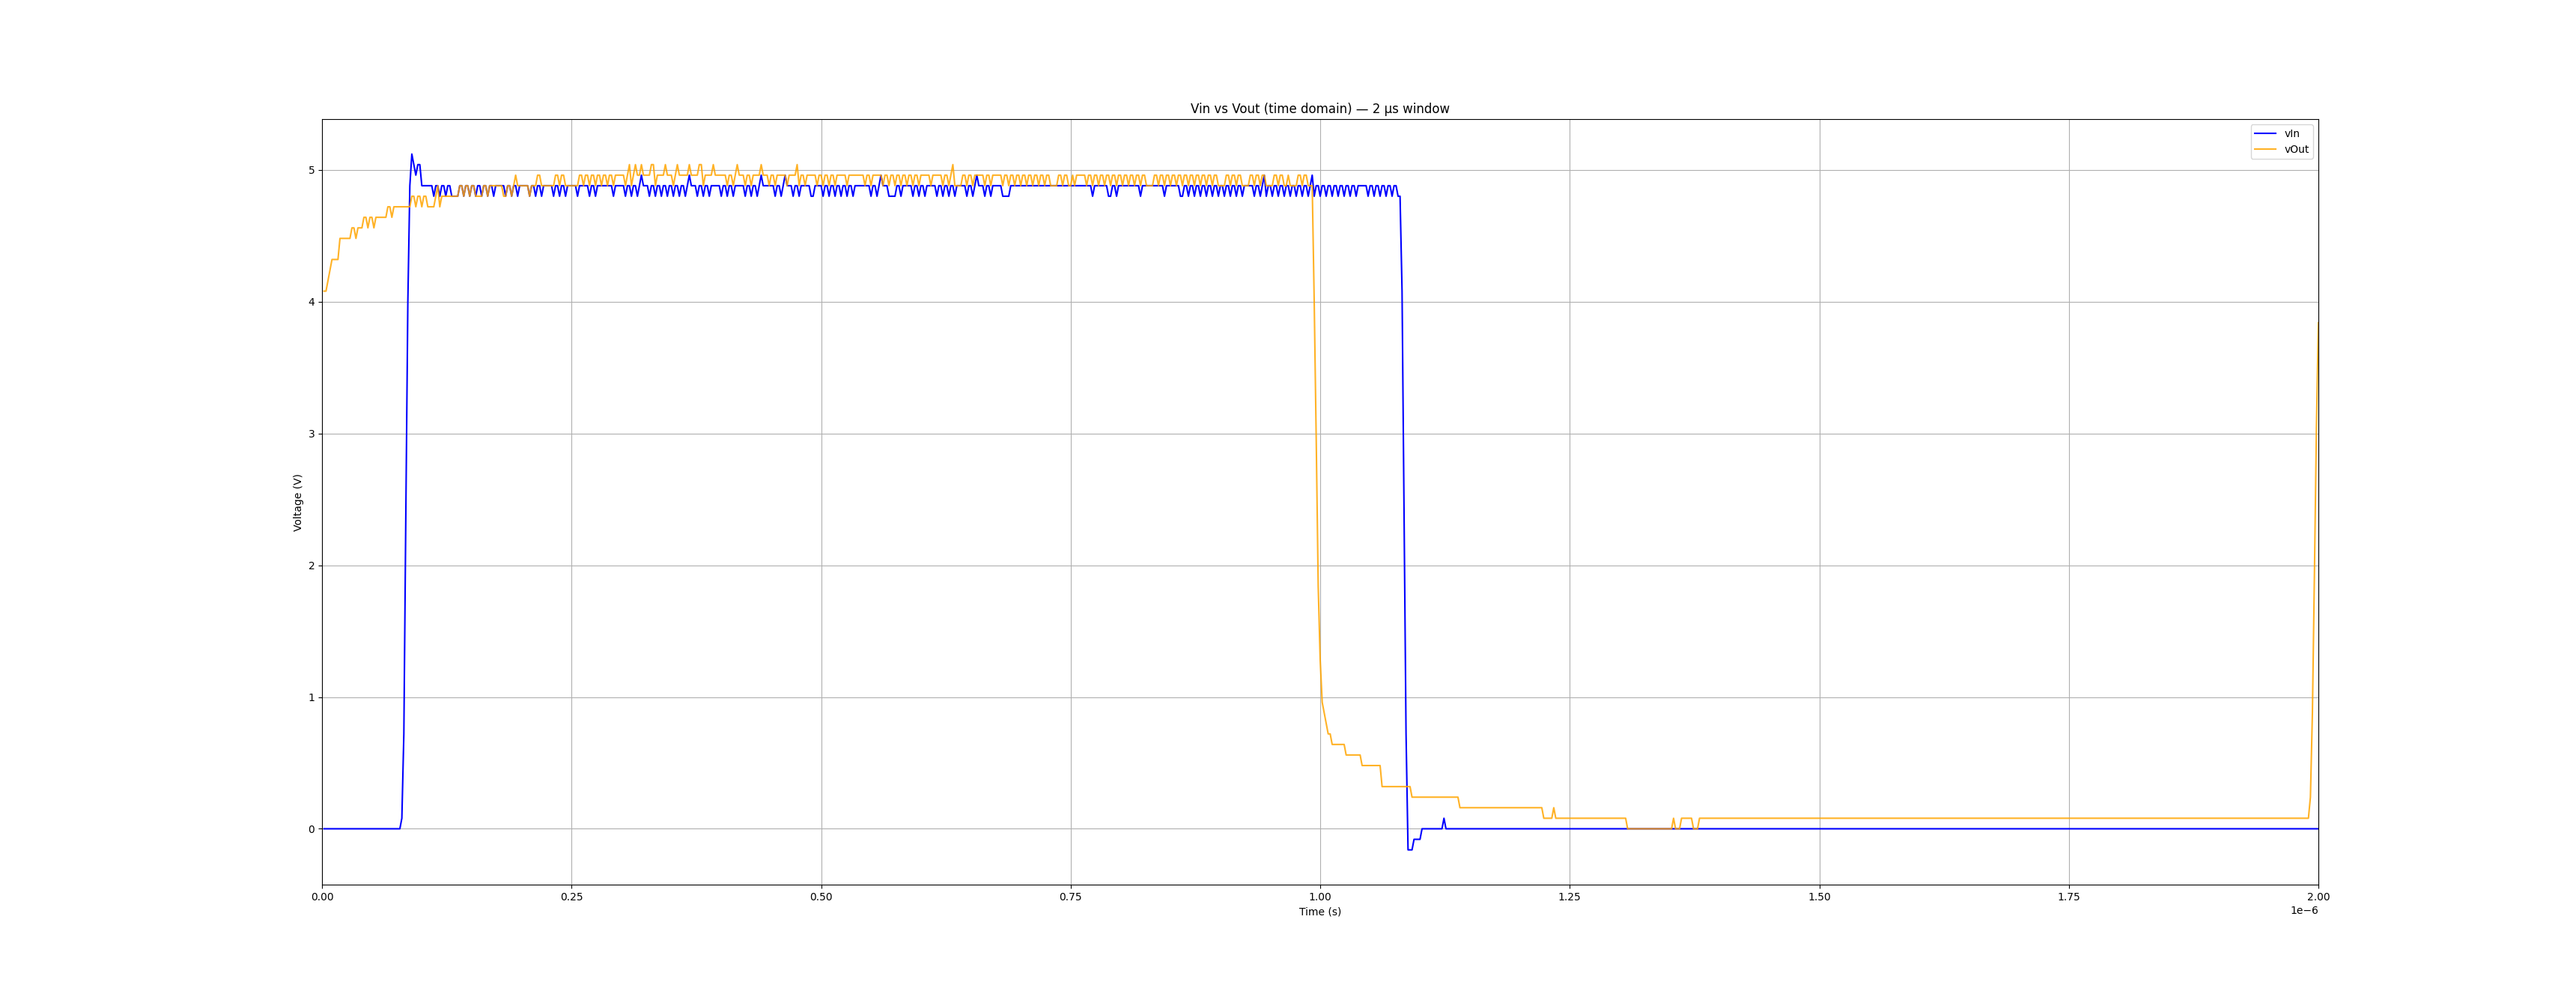
\includegraphics[width=0.55\textwidth]{Media/labShortV.png}
    \textit{
        \caption{Inngangs- og utgangssignaler for 5m koaksialkabel i tidsdomenet.}\label{fig:lab5m_time}}
    
\end{figure}
\subsubsection{Frekvensdomenet} 
Figur \ref{fig:lab5m_freq} viser FFT av inngangs- og utgangssignaler for 5m koaksialkabel i frekvensdomenet. Vi ser at de harmoniske komponentene er tilnærmet uendret, med minimal demping. Dette indikerer at kabelen har liten effekt på signalets frekvensspekter, noe som er forventet for en kort kabel.
\begin{figure}[h]
    \centering
    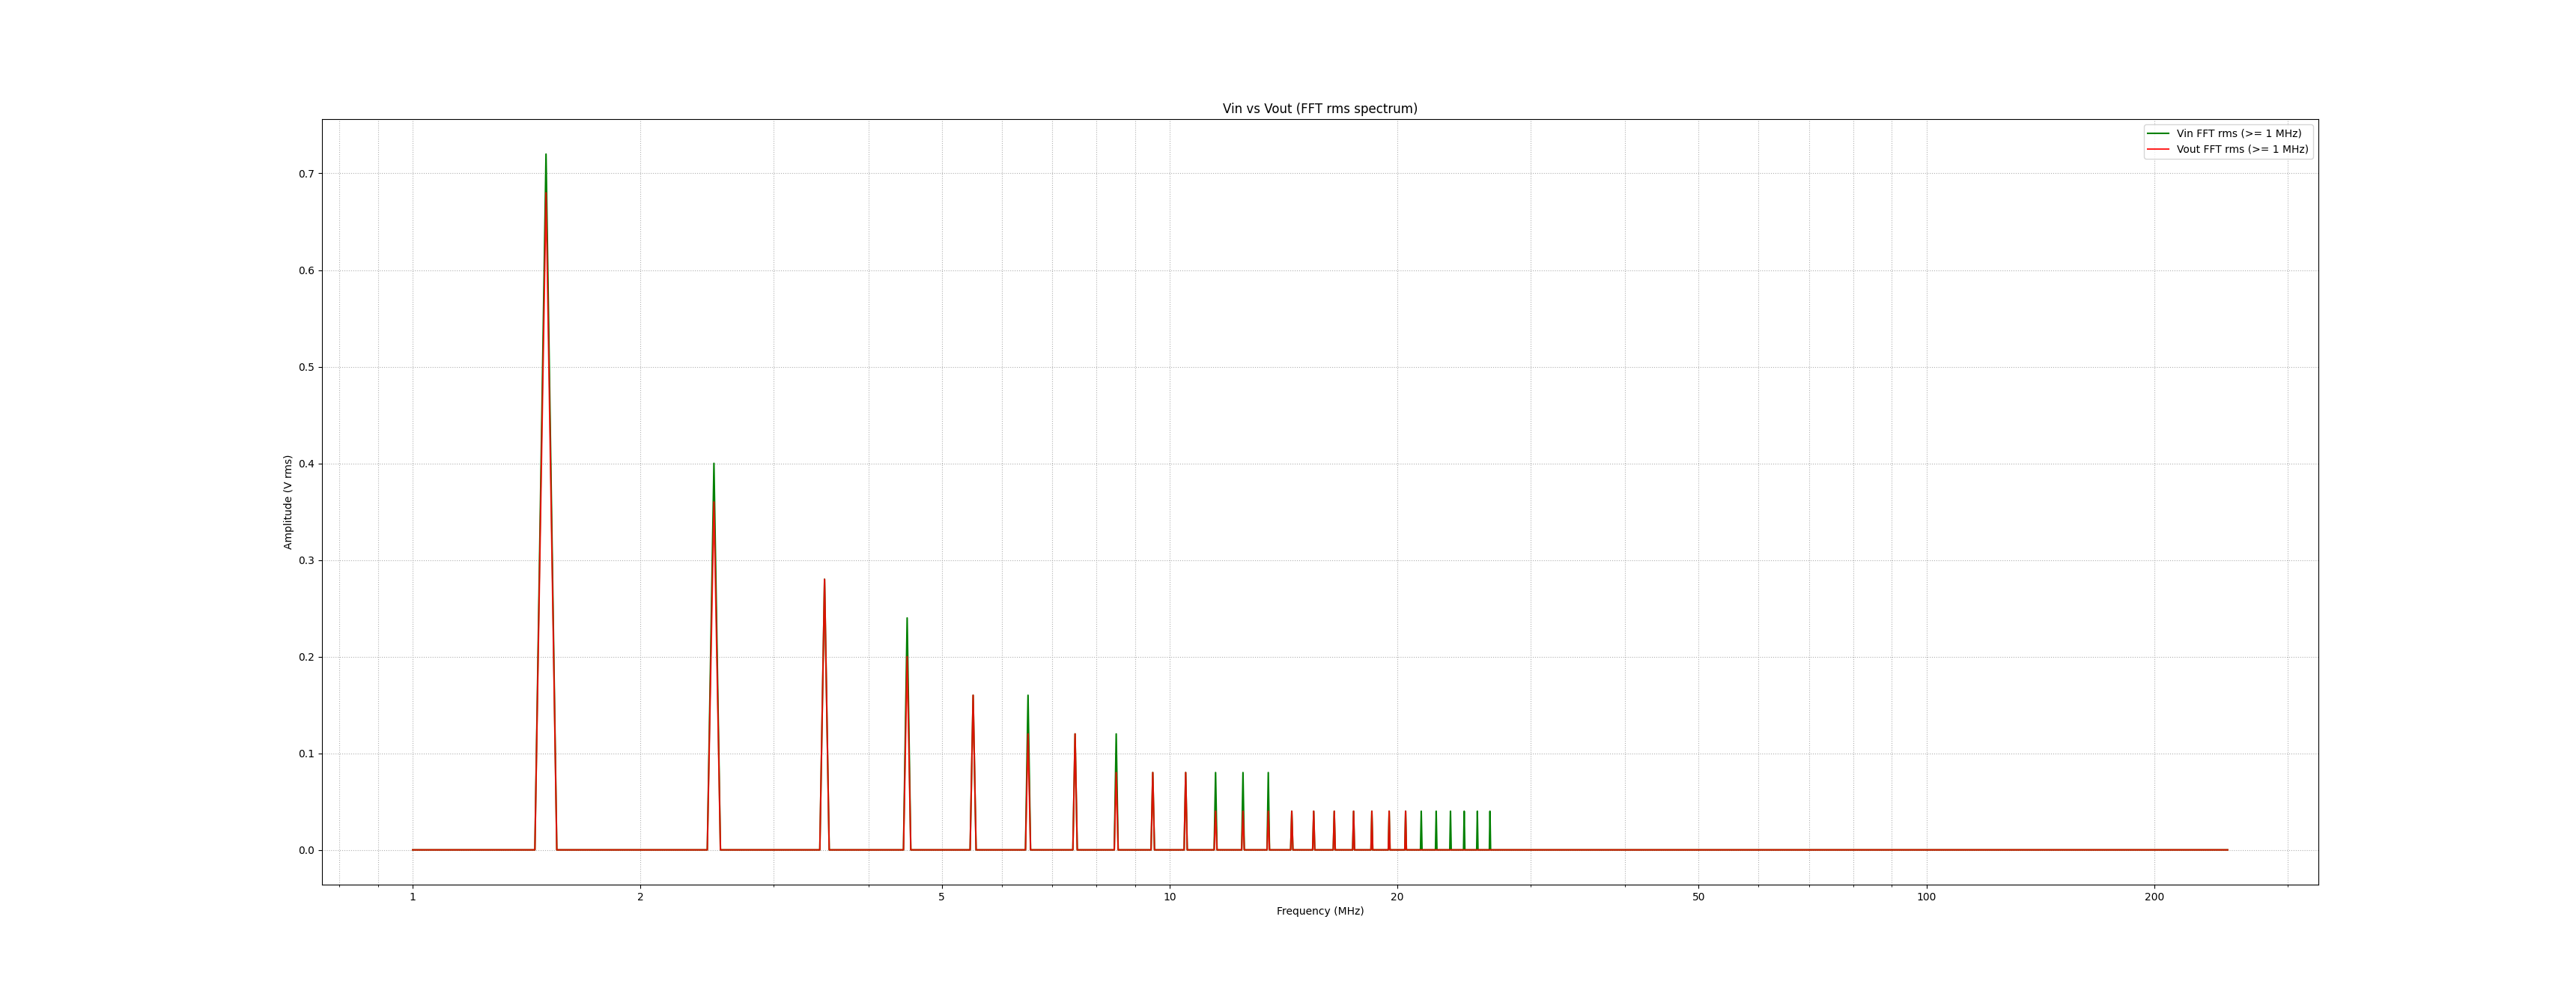
\includegraphics[width=0.6\textwidth]{Media/labShortFreq.png}
    \textit{
        \caption{FFT av inngangs- og utgangssignaler for 5m koaksialkabel i frekvensdomenet.}\label{fig:lab5m_freq}}
    
\end{figure}
\clearpage
\subsection{30m koaksialkabel}
\subsubsection{Tidsdomenet}
Figur \ref{fig:lab30m_time} viser inngangs- og utgangssignaler for 30m koaksialkabel i tidsdomenet. Vi ser at utgangssignalet til en viss grad er dempet og har en liten faseforskyvning sammenlignet med inngangssignalet. Dette er forventet, da forvrengining øker med kabelens lengde.
\begin{figure}[h]
    \centering
    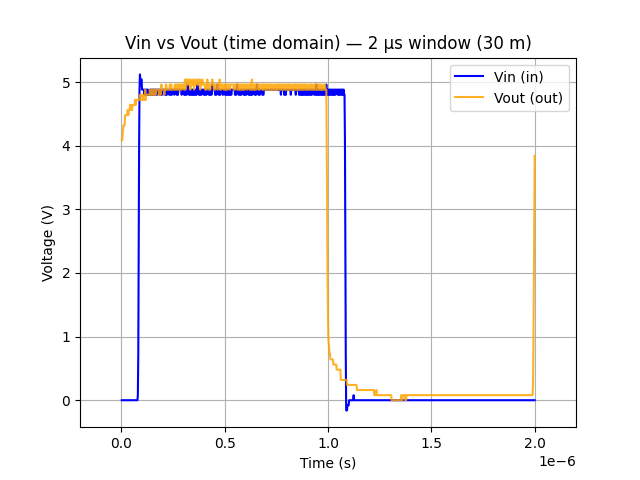
\includegraphics[width=0.6\textwidth]{Media/labLongV.png}
    \textit{
        \caption{Inngangs- og utgangssignaler for 30m koaksialkabel i tidsdomenet.}\label{fig:lab30m_time}}
    
\end{figure}

\subsubsection{Frekvensdomenet}
Figur \ref{fig:lab30m_freq} viser FFT av inngangs- og utgangssignaler for 30m koaksialkabel i frekvensdomenet. Vi ser at de lavere harmoniske komponentene (f.eks. 500 kHz, 1.5 MHz) er relativt uendret, mens de høyere harmoniske komponentene (f.eks. 4.5 MHz og oppover) er merkbart dempet. Dette indikerer at kabelen har en frekvensavhengig demping som påvirker høyfrekvente signaler mer enn lavfrekvente signaler.
\begin{figure}[h]
    \centering
    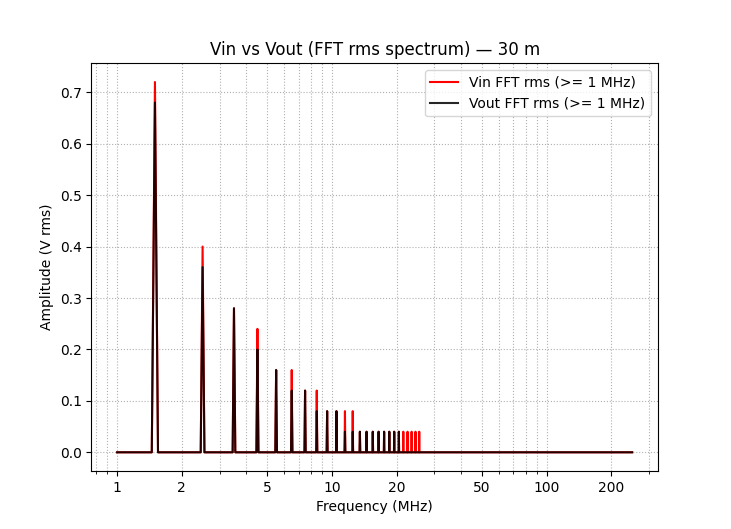
\includegraphics[width=0.6\textwidth]{Media/labLongFreq.png}
    \textit{
        \caption{FFT av inngangs- og utgangssignaler for 30m koaksialkabel i frekvensdomenet.}\label{fig:lab30m_freq}}
    
\end{figure}
